%----------------------------------------------------------------------------
\section{Vector Autoregressions}
%----------------------------------------------------------------------------

\begin{frame}

\begin{center}
{\LARGE Vector Autoregressions}
\end{center}

\end{frame}

%%%%%%%%%%%%%%%%%%%%%%%%%%%%%%%%%%%%%%%%%%%%%%%%%%%%%%%%%%%%%%%%%%%%%%%%%%%%%%
%%%%%%%%%%%%%%%%%%%%%%%%%%%%%%%%%%%%%%%%%%%%%%%%%%%%%%%%%%%%%%%%%%%%%%%%%%%%%%

\begin{frame}{Vector autoregressions (VARs)}

Example: $p$-order VAR in two variables ($y_{t}$ and $x_{t}$)\ldots
\begin{eqnarray*}
y_{t} 	&=& a^{(1)}_{11}y_{t-1}+\ldots +a^{(p)}_{11}y_{t-p}+a^{(1)}_{12}x _{t-1}+\ldots+a^{(p)}_{12}x _{t-p}+u_{yt} \\
x _{t} 	&=&	a_{21}^{(1)}y_{t-1}+\ldots +a^{(p)}_{21}y_{t-p}+a^{(1)}_{22}x_{t-1}+\ldots +a^{(p)}_{22}x _{t-p}+u_{xt}
\end{eqnarray*}
\begin{itemize}
\item[]	where we imagine, say, $y_{t}$ being a measure of real activity and $x_{t}$ a measure of the stance of monetary policy (interest rate or money supply)
\end{itemize}
\vspace{1.5mm}
In matrix form\ldots
\begin{small}
\begin{equation*}
\begin{pmatrix}
y_{t} \\
x_{t}
\end{pmatrix}
= A(L)
\begin{pmatrix}
y_{t-1} \\
x_{t-1}
\end{pmatrix}
+
\begin{pmatrix}
u_{yt} \\
u_{xt}
\end{pmatrix}
\end{equation*}
\end{small}
\begin{itemize}
\item[]	where A(L) is a $p$-order matrix polynomial in the \href{https://en.wikipedia.org/wiki/Lag_operator}{lag operator} and $u_{it}$ is an innovation (`forecast error') to variable $i$.
\end{itemize}

\end{frame}

%%%%%%%%%%%%%%%%%%%%%%%%%%%%%%%%%%%%%%%%%%%%%%%%%%%%%%%%%%%%%%%%%%%%%%%%%%%%%%
%%%%%%%%%%%%%%%%%%%%%%%%%%%%%%%%%%%%%%%%%%%%%%%%%%%%%%%%%%%%%%%%%%%%%%%%%%%%%%

\begin{frame}{Vector Autoregressions}

Consider the special case of a VAR(1) ($p=1$)
\begin{equation*}
\begin{pmatrix}
y_{t} \\
x_{t}
\end{pmatrix}
=
\begin{pmatrix}
a_{11} 	& a_{12} \\
a_{21}	& a_{22}
\end{pmatrix}
\begin{pmatrix}
y_{t-1} \\
x_{t-1}
\end{pmatrix}
+
\begin{pmatrix}
u_{yt} \\
u_{xt}
\end{pmatrix}
\end{equation*}

Thus we have
\begin{eqnarray*}
y_{t} &=& a_{11} y_{t-1} + a_{12}x_{t-1} + u_{yt}	\\
x_{t} &=& a_{21} y_{t-1} + a_{22}x_{t-1} + u_{xt}
\end{eqnarray*}

Let us now consider the `forecast errors', $u_{yt}$ and $u_{xt}$\ldots

\end{frame}

%%%%%%%%%%%%%%%%%%%%%%%%%%%%%%%%%%%%%%%%%%%%%%%%%%%%%%%%%%%%%%%%%%%%%%%%%%%%%%
%%%%%%%%%%%%%%%%%%%%%%%%%%%%%%%%%%%%%%%%%%%%%%%%%%%%%%%%%%%%%%%%%%%%%%%%%%%%%%

\begin{frame}{Vector Autoregressions}

$x_{t}$ may not be what was expected at $t-1$ because 
\begin{itemize}
\item	the policymaker responded to surprises elsewhere in the economy in $t$
\item	the policymaker did something unexpected in a way unrelated to the broader economy (e.g. unexpected change in the voting patterns of a policy committee after new appointments)
\end{itemize}

\vspace{2mm}
We are interested in the effect of a \emph{policy surprise} (i.e. originating with the policymaker) rather than a surprise to the policy instrument, \emph{per se}
\begin{itemize}
\item	\textbf{But} without further assumptions $u_{xt}$ could be a combination of the desired `policy shock' and an `output shock' (such as a random loss in confidence by consumers, say)
\end{itemize}

\end{frame}

%%%%%%%%%%%%%%%%%%%%%%%%%%%%%%%%%%%%%%%%%%%%%%%%%%%%%%%%%%%%%%%%%%%%%%%%%%%%%%
%%%%%%%%%%%%%%%%%%%%%%%%%%%%%%%%%%%%%%%%%%%%%%%%%%%%%%%%%%%%%%%%%%%%%%%%%%%%%%

\begin{frame}{Vector Autoregressions}

$x_{t}$ may not be what was expected at $t-1$ because 
\begin{itemize}
\item	the policymaker responded to surprises elsewhere in the economy in $t$
\item	\textcolor{red}{the policymaker did something unexpected in a way unrelated to the broader economy (e.g. unexpected change in the voting patterns of a policy committee after new appointments)}
\end{itemize}

\vspace{2mm}
We are interested in the effect of a \textcolor{red}{\emph{policy surprise}} (i.e. originating with the policymaker) rather than a surprise to the policy instrument, \emph{per se}
\begin{itemize}
\item	\textbf{But} without further assumptions $u_{xt}$ could be a combination of the desired `policy shock' and an `output shock' (such as a random loss in confidence by consumers, say)
\end{itemize}

\end{frame}

%%%%%%%%%%%%%%%%%%%%%%%%%%%%%%%%%%%%%%%%%%%%%%%%%%%%%%%%%%%%%%%%%%%%%%%%%%%%%%
%%%%%%%%%%%%%%%%%%%%%%%%%%%%%%%%%%%%%%%%%%%%%%%%%%%%%%%%%%%%%%%%%%%%%%%%%%%%%%

\begin{frame}{Vector Autoregressions}

We can think of the forecast errors as being a linear combination of `structural' shocks, $e_{yt}$ and $e_{xt}$ where the latter is the `policy shock'
\begin{equation*}
\begin{pmatrix}
u_{yt} \\
u_{xt}
\end{pmatrix}
=
\begin{pmatrix}
e_{yt}+\theta e_{xt} \\
\phi e_{yt} + e_{xt}
\end{pmatrix}
=
\begin{pmatrix}
1 	& \theta \\
\phi & 1
\end{pmatrix}
\begin{pmatrix}
e_{yt} \\
e_{xt}
\end{pmatrix}
\equiv
B
\begin{pmatrix}
e_{yt} \\
e_{xt}
\end{pmatrix}
\end{equation*}

\vspace{2mm}
Without assumptions on $B$ (i.e. on $\theta$ and $\phi$ in this example) we cannot `pull apart' the forecast errors ($u_{it}$) and separately \textbf{identify} the effect of the structural shocks ($e_{it}$)
\begin{itemize}
\item	Example 1: Assume $\phi=0$
	\begin{itemize}
	\item	Policy variable does not respond contemporaneously to `output shocks'
	\end{itemize}
\item	Example 2: Assume $\theta=0$
	\begin{itemize}
	\item	Policy only affects output with a lag
	\end{itemize}
\item	Identified VAR is commonly referred to as a structural vector autoregression (SVAR)
\end{itemize}

\end{frame}
	
%%%%%%%%%%%%%%%%%%%%%%%%%%%%%%%%%%%%%%%%%%%%%%%%%%%%%%%%%%%%%%%%%%%%%%%%%%%%%%
%%%%%%%%%%%%%%%%%%%%%%%%%%%%%%%%%%%%%%%%%%%%%%%%%%%%%%%%%%%%%%%%%%%%%%%%%%%%%%

\begin{frame}{Vector Autoregressions}

Many identification schemes have been proposed (see Christiano \emph{et al} (1999) and Ramey (2016))
	\begin{itemize}
	\item	Two examples above are a case of using different `Cholesky' orderings
	\item	Ordering not unique and results may depend on ordering
	\item	Should have a plausible story
	\item	Logic extends to multiple shocks but more difficult to imagine a complete ordering
	\end{itemize}
Some famous examples of identification based on ordering\ldots
\begin{itemize}
\item	Sims (1992)
\item	Christiano, Eichenbaum and Evans (2005) - only used one ordering assumption
\end{itemize}

\end{frame}

%%%%%%%%%%%%%%%%%%%%%%%%%%%%%%%%%%%%%%%%%%%%%%%%%%%%%%%%%%%%%%%%%%%%%%%%%%%%%%
%%%%%%%%%%%%%%%%%%%%%%%%%%%%%%%%%%%%%%%%%%%%%%%%%%%%%%%%%%%%%%%%%%%%%%%%%%%%%%

\begin{frame}{Sims (1992)}

Six variable VAR for UK $1965-1990$ with causal ordering
	\begin{enumerate}
	\item Short interest rate ($R$)
	\item Index of foreign exchange value of domestic currency
	\item Commodity price index
	\item Monetary aggregate
	\item Consumer price index
	\item Industrial production index
	\end{enumerate}

\vspace{2mm}
Innovations only affect variables (weakly) lower in causal ordering
	\begin{itemize}
	\item	Interest rate first $\Rightarrow$ Central Bank not contemporaneously reacting to economic news
	\end{itemize}

\end{frame}

%%%%%%%%%%%%%%%%%%%%%%%%%%%%%%%%%%%%%%%%%%%%%%%%%%%%%%%%%%%%%%%%%%%%%%%%%%%%%%
%%%%%%%%%%%%%%%%%%%%%%%%%%%%%%%%%%%%%%%%%%%%%%%%%%%%%%%%%%%%%%%%%%%%%%%%%%%%%%

\begin{frame}{Sims (1992)}

\begin{figure}
\caption[Sims (1992) VAR]{Sims (1992) VAR for U.K. Economy}
\centering
\label{fig:sims_uk}
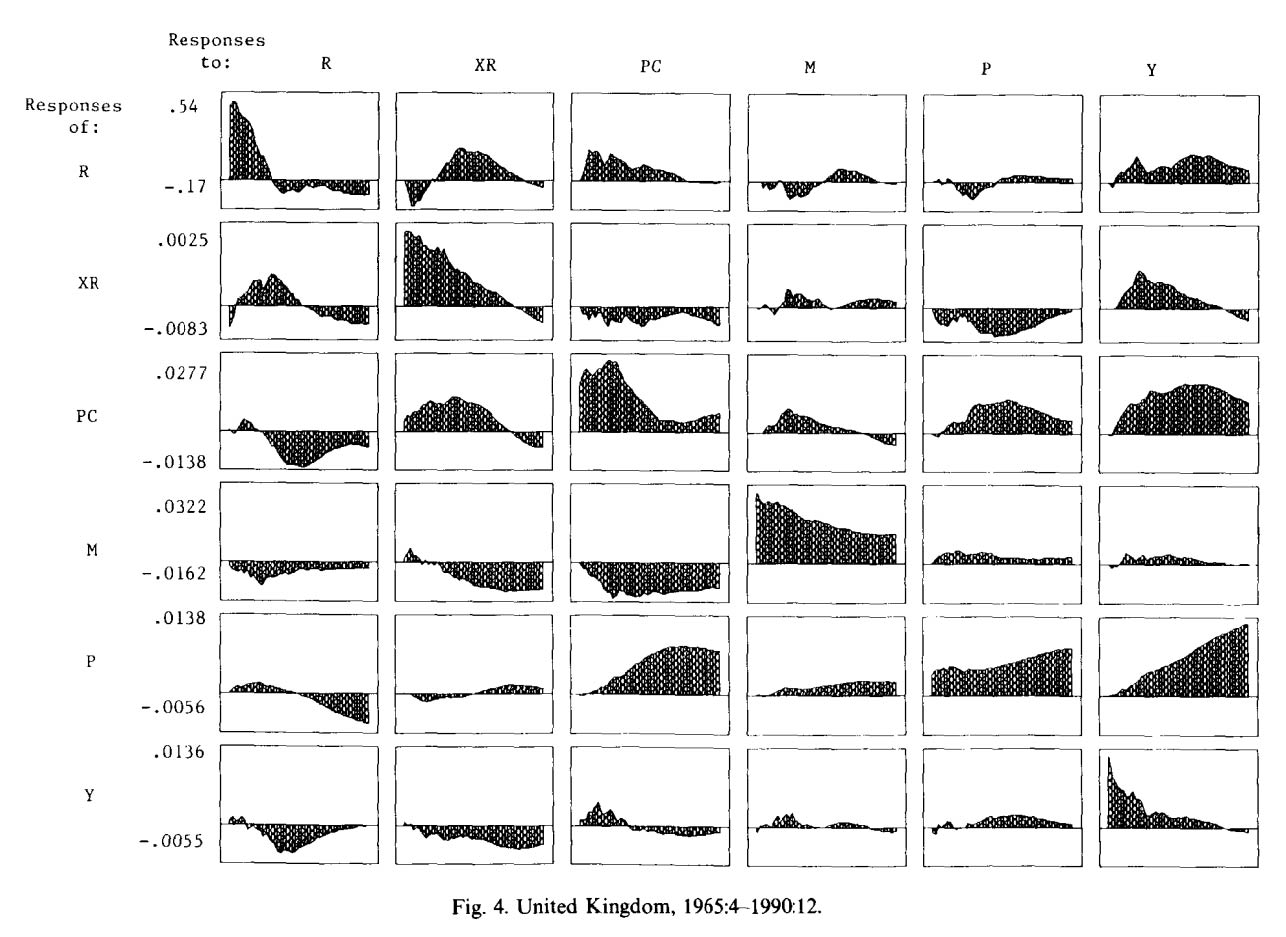
\includegraphics[width=0.65\textwidth]{Figures/sims_uk.JPG}
\end{figure}

\end{frame}

%%%%%%%%%%%%%%%%%%%%%%%%%%%%%%%%%%%%%%%%%%%%%%%%%%%%%%%%%%%%%%%%%%%%%%%%%%%%%%
%%%%%%%%%%%%%%%%%%%%%%%%%%%%%%%%%%%%%%%%%%%%%%%%%%%%%%%%%%%%%%%%%%%%%%%%%%%%%%

\begin{frame}{Christiano, Eichenbaum and Evans (2005)}

Nine variable VAR for US $1965-1995$ with causal ordering
	\begin{enumerate}
	\item 	Real GDP
	\item	Real consumption
	\item	GDP deflator
	\item	Real investment
	\item	Real wage
	\item	Labor productivity
	\item 	Interest rate
	\item 	Real profit
	\item	Growth rate of M2
	\end{enumerate}

Implications of position of $R$:
	\begin{itemize}	
	\item	$R$ Shocks only affect real profit and M2
	\item	$R$ Affected by all shocks except real profit and M2 shocks
	\end{itemize}

\end{frame}

%%%%%%%%%%%%%%%%%%%%%%%%%%%%%%%%%%%%%%%%%%%%%%%%%%%%%%%%%%%%%%%%%%%%%%%%%%%%%%
%%%%%%%%%%%%%%%%%%%%%%%%%%%%%%%%%%%%%%%%%%%%%%%%%%%%%%%%%%%%%%%%%%%%%%%%%%%%%%

\begin{frame}{Christiano, Eichenbaum and Evans (2005)}

Results suggest that after an expansionary monetary policy shock:
\begin{enumerate}
\item 	Output, consumption, and investment respond in a hump-shape, peaking after about one and a half years and returning to pre-shock levels after about three years
\item 	Inflation responds in a hump-shape, peaking after about two years
\item 	Interest rate falls for roughly one year
\item 	Real profits, real wages, and labor productivity rise
\item 	Growth rate of money rises immediately
\end{enumerate}

\end{frame}

%%%%%%%%%%%%%%%%%%%%%%%%%%%%%%%%%%%%%%%%%%%%%%%%%%%%%%%%%%%%%%%%%%%%%%%%%%%%%%
%%%%%%%%%%%%%%%%%%%%%%%%%%%%%%%%%%%%%%%%%%%%%%%%%%%%%%%%%%%%%%%%%%%%%%%%%%%%%%

\begin{frame}{Christiano, Eichenbaum and Evans (2005)}

\begin{figure}
\caption[CEE - Subset 1]{CEE (2005) - Impulse responses (I)}
\centering
\label{fig:cee_responses}
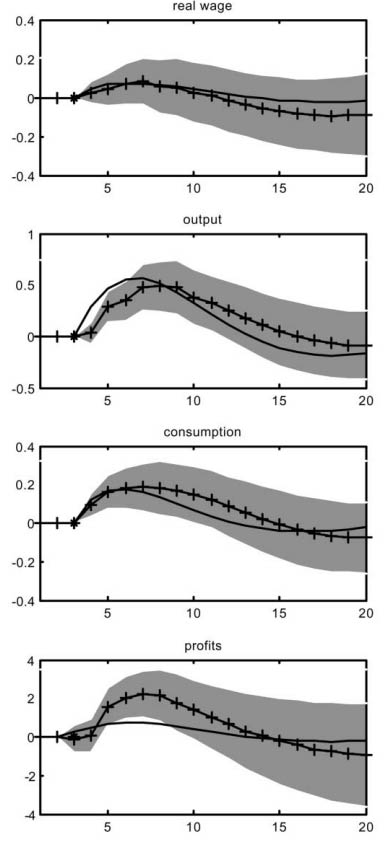
\includegraphics[width=0.25\textwidth]{Figures/cee_responses.JPG}
\end{figure}

\end{frame}

%%%%%%%%%%%%%%%%%%%%%%%%%%%%%%%%%%%%%%%%%%%%%%%%%%%%%%%%%%%%%%%%%%%%%%%%%%%%%%
%%%%%%%%%%%%%%%%%%%%%%%%%%%%%%%%%%%%%%%%%%%%%%%%%%%%%%%%%%%%%%%%%%%%%%%%%%%%%%

\begin{frame}{Christiano, Eichenbaum and Evans (2005)}

\begin{figure}
\caption[CEE - Subset 1]{CEE (2005) - Impulse responses (II)}
\centering
\label{fig:more_cee_responses}
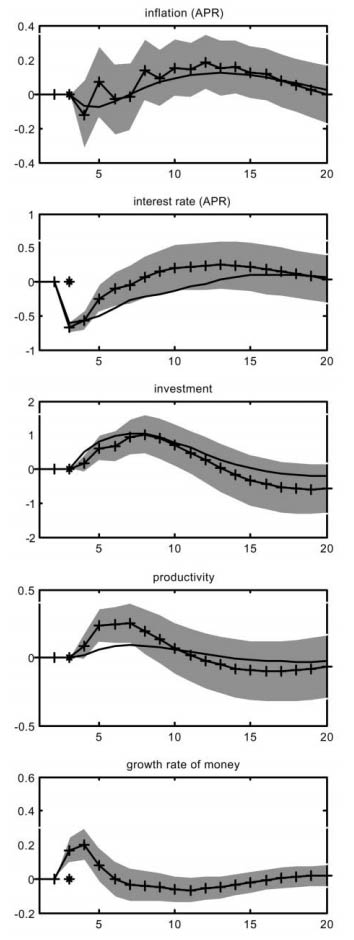
\includegraphics[width=0.20\textwidth]{Figures/more_cee_responses.JPG}
\end{figure}

\end{frame}

%%%%%%%%%%%%%%%%%%%%%%%%%%%%%%%%%%%%%%%%%%%%%%%%%%%%%%%%%%%%%%%%%%%%%%%%%%%%%%
%%%%%%%%%%%%%%%%%%%%%%%%%%%%%%%%%%%%%%%%%%%%%%%%%%%%%%%%%%%%%%%%%%%%%%%%%%%%%%

\begin{frame}{Problems with causal orderings}

Sims (1992) and CEE (2005) find prices initially $\uparrow $ after unexpected $R_{t} \uparrow$
	\begin{itemize}
	\item	Often referred to as the `price puzzle'
	\item 	Could be a cost channel effect (firm borrowing costs rise so they increase prices) but more likely faulty identification	
	\item	Thoughts on other possible explanations?
	\end{itemize}
\vspace{2mm}
Sign restriction VARs designed to rule out such anomalies
	\begin{itemize}
	\item	Impose restrictions not by ordering but by restricting which direction variables should move in following a shock
	\item	See Canova (2007), Canova and Paustian (2010), Uhlig (1998), Rubio-Ramirez (2018)
	\item	Though if the problem is incorrect set of variables (information for forecast) then might not help?
	\end{itemize}

\end{frame}

%%%%%%%%%%%%%%%%%%%%%%%%%%%%%%%%%%%%%%%%%%%%%%%%%%%%%%%%%%%%%%%%%%%%%%%%%%%%%%
%%%%%%%%%%%%%%%%%%%%%%%%%%%%%%%%%%%%%%%%%%%%%%%%%%%%%%%%%%%%%%%%%%%%%%%%%%%%%%

\begin{frame}{Sign restrictions}

\begin{figure}
\caption[Canov 2007]{Canova (2007) - Comparing responses to a monetary tightening based on Cholesky and Sign restrictions}
\centering
\label{fig:sign_vs_chol_irfs}
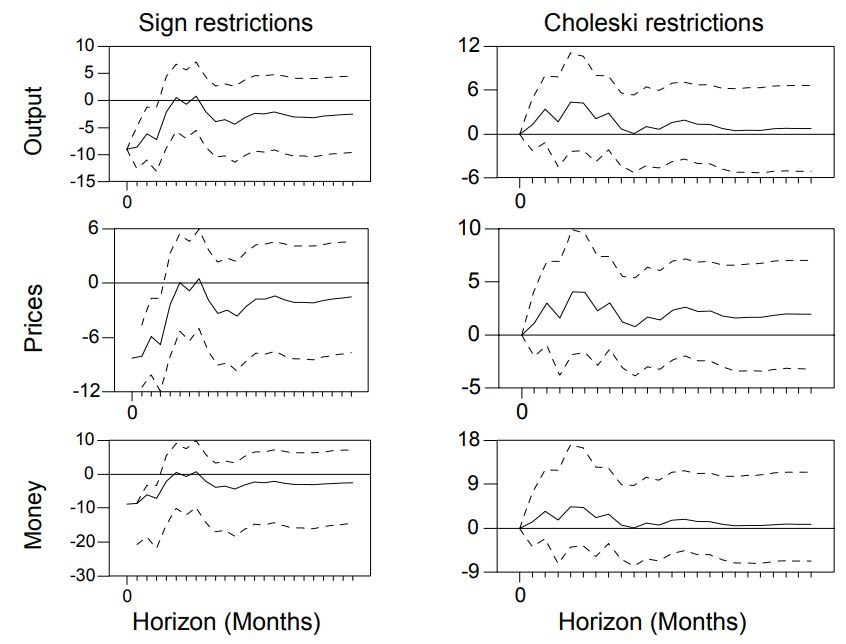
\includegraphics[width=0.60\textwidth]{Figures/sign_vs_chol_irfs.JPG}
\end{figure}

\end{frame}

%%%%%%%%%%%%%%%%%%%%%%%%%%%%%%%%%%%%%%%%%%%%%%%%%%%%%%%%%%%%%%%%%%%%%%%%%%%%%%
%%%%%%%%%%%%%%%%%%%%%%%%%%%%%%%%%%%%%%%%%%%%%%%%%%%%%%%%%%%%%%%%%%%%%%%%%%%%%%

\begin{frame}{Sign restrictions}

\begin{figure}
\caption[Canova and Paustian 2010]{Canova and Paustian (2010) - Sign restrictions}
\centering
\label{fig:sign_restrictions}
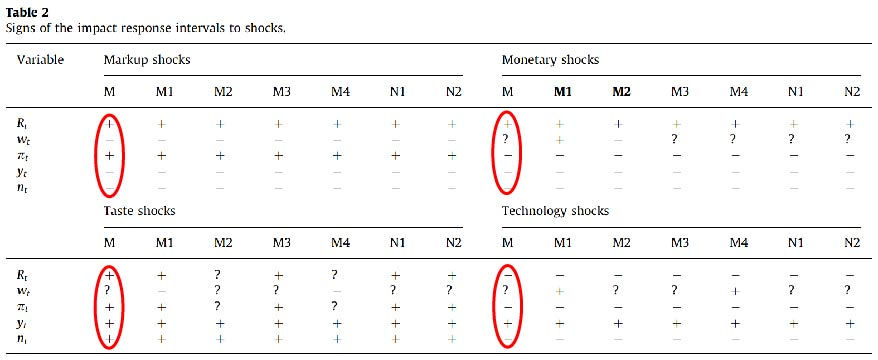
\includegraphics[width=1.0\textwidth]{Figures/sign_restrictions.JPG}
\end{figure}

\end{frame}

%%%%%%%%%%%%%%%%%%%%%%%%%%%%%%%%%%%%%%%%%%%%%%%%%%%%%%%%%%%%%%%%%%%%%%%%%%%%%%
%%%%%%%%%%%%%%%%%%%%%%%%%%%%%%%%%%%%%%%%%%%%%%%%%%%%%%%%%%%%%%%%%%%%%%%%%%%%%%

\begin{frame}{Identification using high frequency information}

\begin{itemize}
\item ECB monthly press conference January 15, 2009
\item Traders expect interest rate cut on February 5, 2009
\item Trichet announces no policy change expected next meeting
\item Traders revise up expectations
\end{itemize}

\end{frame}

%%%%%%%%%%%%%%%%%%%%%%%%%%%%%%%%%%%%%%%%%%%%%%%%%%%%%%%%%%%%%%%%%%%%%%%%%%%%%%
%%%%%%%%%%%%%%%%%%%%%%%%%%%%%%%%%%%%%%%%%%%%%%%%%%%%%%%%%%%%%%%%%%%%%%%%%%%%%%

\begin{frame}{Rosa (2008)}

\begin{figure}
\caption[Rosa (2008)]{Rosa (2008) - Mid-quote on 3-month Euribor future expiring in 03/09}
\centering
\label{fig:trichet_mkt_react}
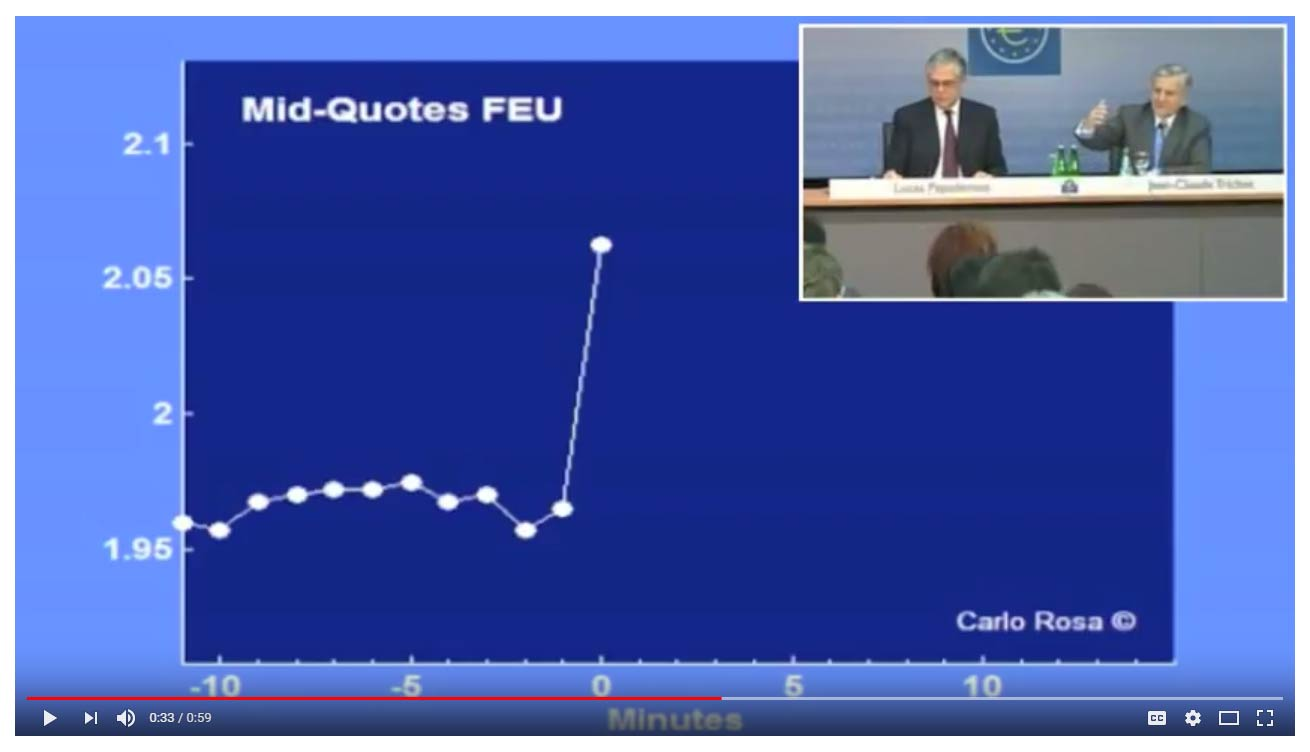
\includegraphics[width=0.45\textwidth]{Figures/trichet_mkt_react.JPG}
\end{figure}

Time zero when Trichet starts answering a journalist's question
\begin{itemize}
\item	Presumption is that nothing else `changes' during the short period from just before to just after $\Rightarrow$ Simply captures policy-surprise
\item	NOTE: Current debate about whether the CB is revealing info about the rest of the economy (as opposed to simply about monetary policy)
\end{itemize}

\end{frame}

%%%%%%%%%%%%%%%%%%%%%%%%%%%%%%%%%%%%%%%%%%%%%%%%%%%%%%%%%%%%%%%%%%%%%%%%%%%%%%%%
%%%%%%%%%%%%%%%%%%%%%%%%%%%%%%%%%%%%%%%%%%%%%%%%%%%%%%%%%%%%%%%%%%%%%%%%%%%%%%%%
%
%\begin{frame}{Kuttner (2001)}
%
%Spot-month futures rate on day $t$ of month $s$ interpreted as conditional expectation of the average funds rate in month $s$ plus term premium
%\begin{equation*}
%f_{s,t}^{0}=E_{t}\frac{1}{m}\sum\limits_{i\in s}r_{i}+\mu_{s,t}^{0}
%\end{equation*}
%
%Policy surprise measure computed from the 1-day change in the spot-month future rate
%\begin{equation*}
%\Delta \tilde{r}_{t}^{u}=\frac{m}{m-t}\left( f_{s,t}^{0}-f_{s,t-1}^{0}\right)
%\end{equation*}
%
%Surprise is proxied by change in futures rate
%\begin{itemize}
%\item	Leads to what is known as a `proxy VAR'
%\end{itemize}
%
%\end{frame}
%
%%%%%%%%%%%%%%%%%%%%%%%%%%%%%%%%%%%%%%%%%%%%%%%%%%%%%%%%%%%%%%%%%%%%%%%%%%%%%%%%
%%%%%%%%%%%%%%%%%%%%%%%%%%%%%%%%%%%%%%%%%%%%%%%%%%%%%%%%%%%%%%%%%%%%%%%%%%%%%%%%
%
%\begin{frame}{Proxy VAR}
%
%Correlated with both reduced form residuals but with only one structural innovation
%\begin{itemize}
%\item[] $E(e_{yt}z_{t})=\phi $
%\item[] $E(e_{xt}z_{t})=0$
%\end{itemize}
%\begin{equation*}
%\; \; \; \; \:E\left[ \left( 
%\begin{array}{c}
%u_{yt} \\ 
%u_{xt}
%\end{array}
%\right) z_{t}\right] =E\left[ \left( 
%\begin{array}{cc}
%\theta _{1} & \theta _{2} \\ 
%\theta _{3} & \theta _{4}
%\end{array}
%\right) \left( 
%\begin{array}{c}
%e_{yt} \\ 
%e_{xt}
%\end{array}
%\right) \left( \phi e_{yt}+\nu _{t}\right) \right] =\left( 
%\begin{array}{c}
%\theta _{1}\phi \\ 
%\theta _{3}\phi
%\end{array}
%\right)
%\end{equation*}
%
%\vspace{3mm}
%Thus, proxy VAR\ identified by restriction\ldots
%\begin{equation*}
%\frac{\theta _{1}}{\theta _{3}}=\frac{E(u_{yt}z_{t})}{E(u_{xt}z_{t})}
%\end{equation*}
%\begin{itemize}
%\item[] for known $E(u_{yt}z_{t})$ and $E(u_{xt}z_{t})$ (can be estimated from the reduced form VAR residuals and the constructed instrument, $z_{t}$)
%\end{itemize}
%
%\end{frame}

%%%%%%%%%%%%%%%%%%%%%%%%%%%%%%%%%%%%%%%%%%%%%%%%%%%%%%%%%%%%%%%%%%%%%%%%%%%%%%
%%%%%%%%%%%%%%%%%%%%%%%%%%%%%%%%%%%%%%%%%%%%%%%%%%%%%%%%%%%%%%%%%%%%%%%%%%%%%%

\begin{frame}{Vector Autoregressions}

\begin{quotation}
While researchers have disagreed on the best means of identifying policy shocks, there has been a surprising consensus on the general nature of the economic responses to monetary policy shocks. A variety of VARs estimated for a number of countries all indicate that, in response to a policy shocks, output follows a hump-shaped pattern in which the peak impact occurs several quarters after the initial shock.
\end{quotation}
\center - Walsh, 1998, p.31

\end{frame}

%%%%%%%%%%%%%%%%%%%%%%%%%%%%%%%%%%%%%%%%%%%%%%%%%%%%%%%%%%%%%%%%%%%%%%%%%%%%%%%
%%%%%%%%%%%%%%%%%%%%%%%%%%%%%%%%%%%%%%%%%%%%%%%%%%%%%%%%%%%%%%%%%%%%%%%%%%%%%%%
%
%\begin{frame}{Vector Autoregressions}
%
%VAR approach useful but not without flaws/critics\ldots
%\vspace{2mm}
%\begin{itemize}
%\item 	Monetary policy shocks are now likely rare/small (Ramey (2016))
%	\begin{itemize}
%	\item	Makes it more difficult to use \emph{policy} shocks to estimate impact of policy
%	\item	Can still estimate role of policy but need \emph{other} shocks \textbf{and} a model
%	\end{itemize}
%\vspace{1mm}
%\item	Changes in underlying parameters (Lucas critique and Rational Expectations)
%	\begin{itemize}
%	\item	Response to shocks depends on parameters describing policymakers' approach \textbf{and} all other parameters in the economy (e.g. regulation, preferences\ldots)
%	\item	If they change, previous estimates may become obsolete
%	\end{itemize}
%\vspace{1mm}	
%\item 	Responses may not be accurately recovered even from data generated by a model (Chari \emph{et al} (2008))
%	\begin{itemize}
%	\item	Can still use, but in a `moment matching' exercise \emph{involving a model}
%	\item	VARs on actual data and on data from model - minimize discrepancy
%	\end{itemize}
%\end{itemize}
%
%\end{frame}
%
%%%%%%%%%%%%%%%%%%%%%%%%%%%%%%%%%%%%%%%%%%%%%%%%%%%%%%%%%%%%%%%%%%%%%%%%%%%%%%%
%%%%%%%%%%%%%%%%%%%%%%%%%%%%%%%%%%%%%%%%%%%%%%%%%%%%%%%%%%%%%%%%%%%%%%%%%%%%%%%
%
%\begin{frame}{Vector Autoregressions}
%
%More problems with VAR analysis\ldots
%\vspace{2mm}
%\begin{itemize}
%\item	Unhelpful for welfare analysis
%	\begin{itemize}
%	\item	Knowing that policy affects activity is one thing\ldots
%	\item 	\ldots but knowing \emph{how it should try to affect it} is another
%	\item 	Agent's optimization problems must be explicit for micro-founded welfare analysis
%	\item 	VARs are silent on this
%	\end{itemize}
%\item	Story telling / incorporation of microeconomic evidence
%	\begin{itemize}
%	\item 	Policymakers like to understand/explain transmission mechanism
%	\item	Elements of models (such as, say, household risk aversion) can be pinned down by evidence from experiments/more granular research
%	\item	Not possible with VARs (or very difficult)
%	\end{itemize}
%\end{itemize}
%
%\vspace{2mm}
%A lot of these `problems' can be addressed by using a model\ldots
%
%\end{frame}

